\documentclass[letter,10pt]{article}
\usepackage[utf8]{inputenc}
\usepackage[english]{babel}
\usepackage{fancyvrb}
\usepackage{fancyhdr}
\usepackage{url}
\usepackage{verbatim}
\usepackage{graphicx}
\usepackage{rotating}
\usepackage{listings}
\usepackage{float}


\lstset{
language=C
}

\parskip 1mm
\setlength{\topmargin}{0pt}
\oddsidemargin  0.5cm
\evensidemargin 0.5cm
\textwidth      15.5cm
\textheight     21.0cm
\headsep        4 mm
\parindent      0.5cm

\pagestyle{fancyplain}

\lhead{Estadística Computacional 2015}
\rhead{\bf \it LEC 1 }
\lfoot{}
\cfoot{}
\rfoot{\bf \thepage}
\renewcommand{\footrulewidth}{0.4pt}

\title{LEC1 \\ Estadística Computacional 2015-1, UTFSM }
\author{Gonzalo Moya 201173016-k}

\date{\vspace*{1cm} Valparaíso, 30 de Octubre del 2015}

\newpage

\begin{document}
\maketitle
\thispagestyle{empty}
\newpage
\tableofcontents

\makeatother

\newpage

\section{Introducción}
El presente documento abarca el estudio sobre distintas variables de una data relacionada con vehículos y alguna de sus características con el fin de realizar 
un estudio que busque encontrar relaciones entre las distintas variables y a partir de ello concluir a qué pueden deberse o bien ayudar en la toma de alguna decisión 
que involucre la internalización de aquellas variables en algun problema.

\section{Desarrollo}
\subsection{Pregunta 1}

Para estudiar la dispersión de las variables se construye una tabla con la desviación estandar $(S)$, la media $(X)$ y el coeficiente
de variación $(C_v)$.

\begin{table}[h]
    \begin{center}
    \begin{tabular}{|l|l|l|l|}
    \hline
    Variable     & $S$ & $X$ & $C_{v}$ \\ \hline
    mpg          & 7.815984 & 23.51457 & 0.332389 \\
    cylinders    & 1.701004 & 5.454774 & 0.3118377 \\
    displacement & 104.2698 & 193.4259 & 0.5390687 \\
    horsepower   & 38.26078 & 104.2638 & 0.3669613 \\
    weight       & 846.8418 & 2970.425 & 0.2850912 \\
    acceleration & 2.757689 & 15.56809 & 0.1771373 \\
    model year   & 3.697627 & 76.01005 & 0.04864655 \\
    origin       & 0.8020549 & 1.572864 & 0.5099327 \\ \hline
    \end{tabular}
    \end{center}
\end{table}

Si bien se podría analizar la varianza o la desviación estándar para cada variable esto haría mas engorroso el estudio ya que
todas las variables no estan en medidas similares por lo que comparar el valor de una con la otra directamente no nos permite discrimnar
cual variable podría ser mas exacta. Para contrarestar lo anterior se utiliza el coeficiente de variación el cual a través de la división
entre la desviación estándar y la norma permite entregar valores que se mueven entre 0 y 1, los que además se encuentran normalizados
por las medias de cada variable que se preocupa de hacer el ajuste para el análisis de variables con valores tan distintos como es el presente caso.
Una vez encontrados todos los coeficientes de variación se debe analizar los valores más cercanos a 0. Entre ellos la más homogénea
termina siendo el año de los modelos, lo cual se podía sospechar a simple inspección de la data a través del sumario de cada variable
ya que el año del modelo se mueve entre 70 y 82 a diferencia de otras que tienen grandes valores dentro de sus dominios.


\subsection{Pregunta 2}

Para analizar este punto es necesario ver como se ha comportado la cantidad de autos a través del tiempo,
en este ámbito lo mejor que podemos hacer es utilizar un histograma.

\begin{figure}[h!]
    \centering
    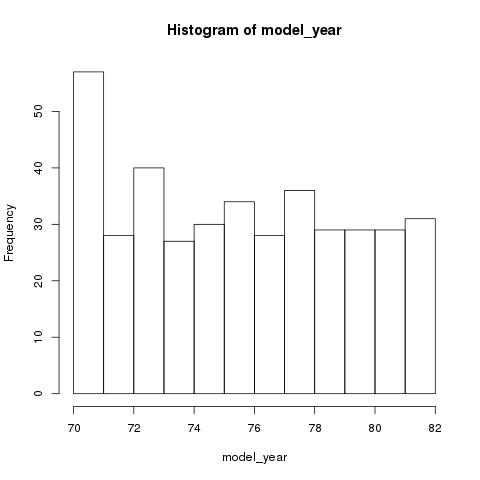
\includegraphics[scale=0.4]{model_year_histogram.jpg}
    \caption{Histograma de cantidad de modelos por año}
    \label{fig:model_year_histogram}
\end{figure}

Observando el gráfico es posible notar que entre los años 70 y 78 existe cierta irregularidad en la cantidad de modelos por
año, logrando la estabilidad desde el 78 en adelante. Las razones que puedan explicar esto son múltiples por ejemplo en aquellos años
no existía la renovación del vehículo por parte de cada dueño cada 1 o 2 años como ocurre hoy en día, además en los años 70 aún
era un mercado emergente que no permitía proyectar bien la demanda.

\newpage

\subsection{Pregunta 3}

Intuitivamente se puede creer que una cilindrada alta implicaría un mayor número de cilindros en el motor,
pero eso no es suficiente para el análisis por lo que es necesario realizar boxplots
donde en un eje se encuentren la cilindrada y en otro la cantidad de cilindros con el fin
de partir el conjunto de cilindrada en grupos por cilindro ilustrados por los diagramas.
\begin{figure}[h!]
    \centering
    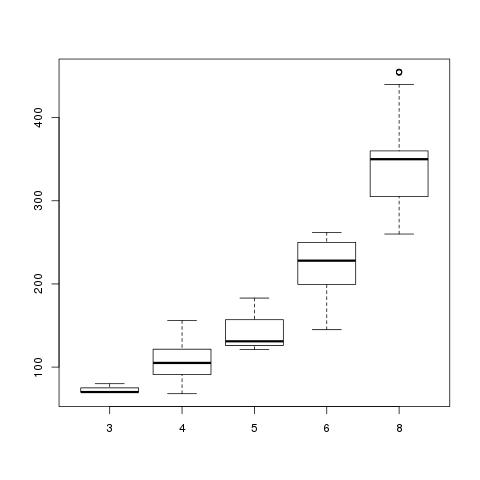
\includegraphics[scale=0.4]{boxplot_displacement_cylinders.jpg}
    \caption{Boxplot de Cilindrada agrupado por Cilindros}
    \label{fig:boxplot_displacement_cylinders}
\end{figure}
A primera vista es posible observar que a medida que se aumentan los cilindros es posible
encontrar motores con mayor cilindradas. La mayoría de las cajas se encuentran acopladas solo por los bigotes lo que muestra
que existe una posible separación entre cada grupo de cilindros y la cilindrada posible pero es importante destacar que esto
no es una separación estricta sino que solamente la concentración de los datos entre cada grupo se encuentra distante donde los bigotes
permiten realizar la ``unión'' entre el conjunto de datos de cada boxplot lo cual indica que estos serían una cantidad mínima
de datos en relación a las cajas en si.
Otro elemento importante es que se puede observar una relación lineal con pendiente positiva entre los boxplot pero
la simple inspección no es suficiente por lo que se calculará la covarianza entre estas dos variables. La covarianza es
168.6232, al ser positiva implica una relación proporcional entre ambas variables por lo que las observaciones a partir
de los boxplot coinciden hasta cierto punto, pero la covarianza no nos entrega la intensidad de la relación por lo que se realiza
el cálculo de otra herramienta dispnonible hasta el momento, la cual es la correlación lineal, con un valor de 0.9507214
positiva y muy cercana a 1 implica una intensidad fuerte en la proporcionalidad entre los cilindros y la cilindrada de los modelos.
\begin{figure}[h!]
    \centering
    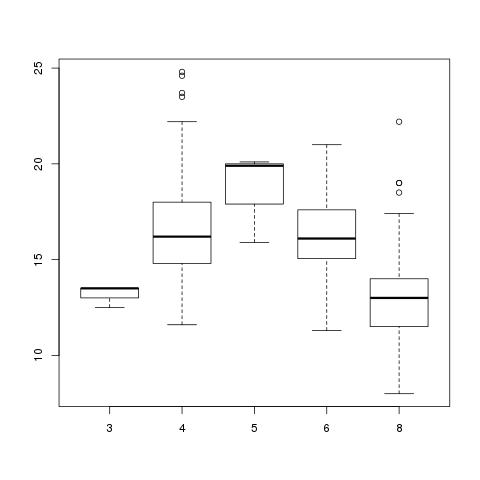
\includegraphics[scale=0.4]{boxplot_acceleration_cylinders.jpg}
    \caption{Boxplot de Aceleración agrupada por Cilindros}
    \label{fig:boxplot_horsepower_cylinders}
\end{figure}

Los boxplot aparentemente tienden a converger hacia el número de cilindros igual a 5 en donde se alcanzan las mayores aceleraciones. Otras características
interesantes son que el boxplot que corresponde a 3 cilindros o  bien tiene muy pocos datos o la variación entre sus valores es demasiada baja lo que demuestra
que tiene una concentración en un rango muy acotado. Los de 4 y 8 cilindros prsetentan datos atípicos pero con gran dispersión entre el resto de sus valores.
Una hipótesis a comprobar es si la dispersión o la cantidad de datos de los boxplot relacionados a 6 y 8 cilindros podrán hacer mas peso que la de los 3 y 4 cilindros.


 Para acompañar la argumentación anterior se calcula la covarianza, esta es de $-2.370842$, al ser negativa entonces
 implica una relación inversamente proporcional 
 reafirmando gran parte de lo dicho anteriormente pero es necesario conocer su intensidad, por lo que se utilizará 
 la correlación lineal, siendo $-0.5054195$. Al encontrarse entre $-1$ y $0$ no es tan fácil afirmar que
 tan fuerte es la intensidad de la relación. Tal vez otro indicador que no busque ajustar mediante alguna recta los datos nos
 podría entregar una relación más precisa.
 


\newpage

\subsection{Pregunta 4}
Del resumen de los datos se desprende que el tercer cuartil es 125, y que el valor máximo es 238, por lo que
los boxplot que muestren valores entre estos dos números podrán asegurar tener las potencias más altas.
\begin{figure}[h!]
    \centering
    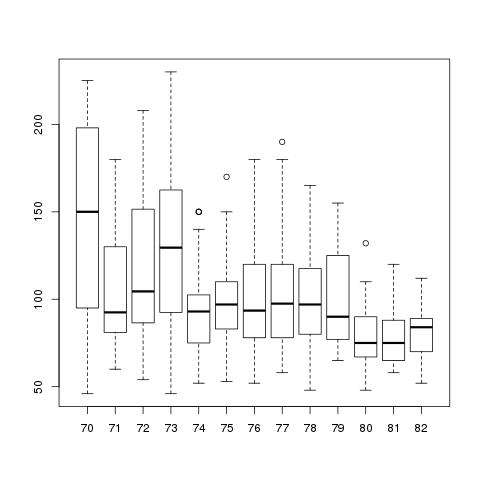
\includegraphics[scale=0.5]{boxplot_horsepower_model_year.jpg}
    \caption{Boxplot de Potencia agrupado por año del modelo}
    \label{fig:boxplot_horsepower_model_year}
\end{figure}

En este grupo se encuentran todos, pero si no contamos los bigotes entonces se consideran los años
entre el 70 y el 79 como los con mayores potencias, la primera idea al respecto es que la modernización tanto de la construcción
de vehículo como de la eficiencia de los motores puede permitir que a través de los años se requiera menos potencia para que estos
puedan moverse adecuadamente. Pero de este gran conjunto de años algunos presentan datos atípicos, estos son el 74, 75 y 77 además desde el 74 en adelante existe
mucha diferencia entre los valores que alcanzan las cajas sin contar los bigotes respecto los que se encuentran en el 70-73, por lo que quedan descartados los del 74 en adelante.
Ahora el grupo en cuestion está entre el 70 y el 73, pero si se observan detenidamente es posible ver que existen dos grupos uno con mayor potencia que el otro, 
notando que la diferencia entre sus medianas es alta sumado a que que los del 71 y 72
concentran la mayor parte de sus datos en valores mucho menores que los del 70 y 73.
Finalmente se concluye que el rango de años con mayor potencia es el 70-73 pero los años con modelos de mayor potencia son específicamente el 70 y el 73.

\newpage
\subsection{Pregunta 5}

Para encontrar este grupo, se decide particionar el consumo en base al origen, luego se realizan boxplot de cada nuevo grupo
permitiendo observar relaciones directas entre origen y el consumo que hay segun este.
\begin{figure}[h!]
    \centering
    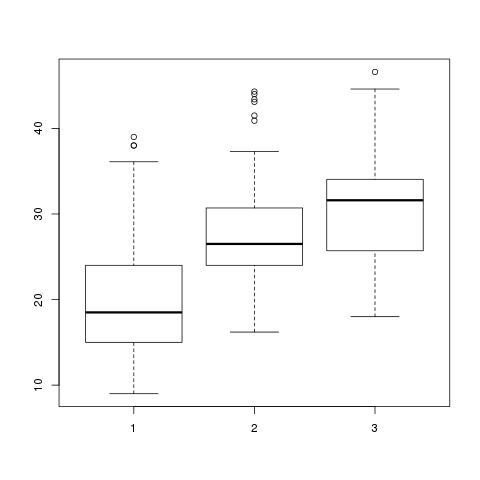
\includegraphics[scale=0.5]{boxplot_mpg_origin.jpg}
    \caption{Boxplot de Consumo de combustible agrupado por origen}
    \label{fig:boxplot_mpg_origin}
\end{figure}
A primera vista se descarta el boxplot que corresponde a los modelos de origen 3, ya que este presenta una concentración de datos en valores
mayores a 30, lo que supera fácilmente a los de origen 1 y 2.
De los restantes se observa que el los que corresponden al origen 1 poseen menor consumo que los del grupo 2, sin ahondar mucho,
el largo de los bigotes de la caja 2 puede hacer pensar que podría llegar a ponderar menos consumo ayudado de su concentración de datos
en sus valores menores, pero para ello necesitaría que la caja estuviera menos desacoplada respecto a la primera, ya que cuando termina una empieza la otra,
dejando a la del grupo de origen 2 sin oportunidad. Por lo tanto los vehículo correspondientes al origen 1 son los de menor consumo.

\newpage
\subsection{Pregunta 6}

Para encontrar la respuesta es necesario realizar una partición de la aceleración y de la potencia, ambas respecto al origen, luego graficar los resultados
mediante boxplots tomando en consideración los que corresponden al origen 1.

  \begin{minipage}{\linewidth}
      \centering
      \begin{minipage}{0.45\linewidth}
          \begin{figure}[H]
              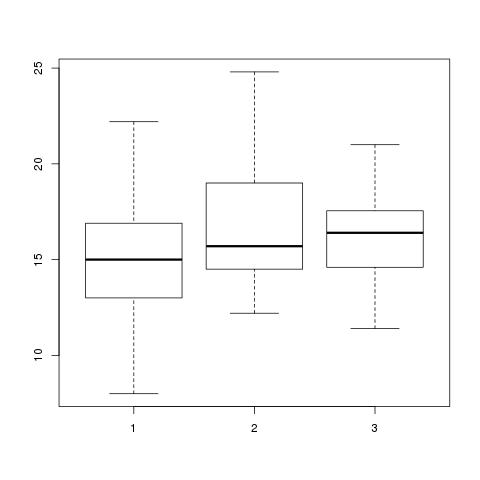
\includegraphics[width=\linewidth]{boxplot_acceleration_origin.jpg}
              \caption{Boxplot de Aceleración agrupado por Origen}
          \end{figure}
      \end{minipage}
      \hspace{0.05\linewidth}
      \begin{minipage}{0.45\linewidth}
          \begin{figure}[H]
              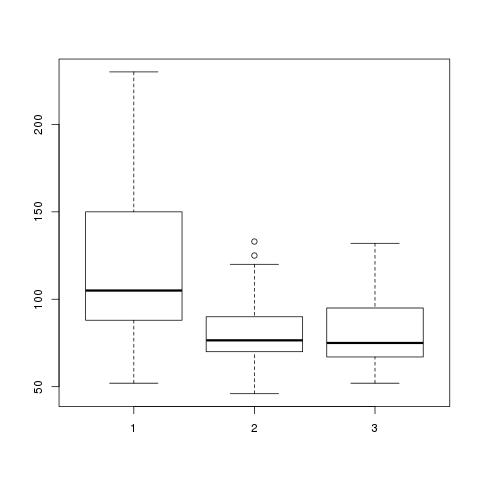
\includegraphics[width=\linewidth]{boxplot_horsepower_origin.jpg}
              \caption{Boxplot de Potencia agrupado por Origen}
          \end{figure}
      \end{minipage}
  \end{minipage}
De ambos, se puede notar que  tanto en aceleración como en potencia los vehículos de origen 1 abarcan casi la totalidad de los
valores posibles en la muestra, lo que podría dificultar el análisis. Pero para resolver esto se debe obervar que el que corresponde a la potencia
posee una concentración de sus datos sus valores menores pero sus cuartiles abarcan datos altos y bajos.
Para hacer un análisis más preciso se obtienen la covarianza, la cual es de $-78.31126$, de esto se entiende que existe una relación inversamente proporcional,
pero se requiere de otro indicador para encontrar la intensidad de esta relación, para ello se usa el coeficiente de correlación lineal, que retorna un valor de 
$-0.7160874$, al ser negativo pero más cercano al -1 que al 0 entonces es posible concluir que la relación es lineal inversamente proporcional.

\newpage
\subsection{Pregunta 7}

De lo desarrollado anteriormente se toman las siguientes condiciones que deben cumplir los modelos:
\begin{itemize}
 \item Cantidad de cilindros igual a 5 y año 70.
 \item Cantidad de cilindros igual a 5 y año 71.
 \item Cantidad de cilindros igual a 5 y año 72.
 \item Cantidad de cilindros igual a 5 y año 73.
\end{itemize}

Al aplicarlas sobre el consumo se obtienen 4 nuevos conjuntos de datos, pero todos estos están vacíos lo que quiere decir que no existen vehículos
con cantidad de cilindros igual a 5 entre los años 70 al 73. Para contrarestar esta situación, es posible volver al boxplot de potencia y años de los modelos, 
con el fin de ampliar el conjunto de vehículos que se encuentran entre los que tienen la mayor potencia, teniendo en cuenta que ahora se toma un intervalo de años
más grande siendo este desde el 70 al 79, por lo que ahora hay que buscar si existen modelos con cantidad de cilindros igual a 5 entre los años 74 al 79. Al separar año
a año se desprende que solo hay dos de estos modelos, perteneciendo a los años 78 y 79. Resumiendo:
\begin{itemize}
 \item Cantidad de cilindros igual a 5 y año 78: Consumo (mpg) igual a 20.3.
 \item Cantidad de cilindros igual a 5 y año 79: Consumo (mpg) igual a 25.4.
\end{itemize}

Ahora están las condiciones para afirmar que el consumo menor es de 20.3 para el año 78, con una diferencia de 5.1 respecto al modelo que le sigue
con un consumo de 25.4 en el año 79.


\subsection{Pregunta 8}
Para responder esta pregunta se tomará el supuesto en que el ayudante Rodrigo Naranjo es amante del derrape en los autos además de ser jugador de cartas Mitos y Leyendas
por lo que necesita ahorrar para poder comprar las mejores cartas. Por tanto, la mejor opción para Rodrigo es el auto mas barato posible y con la mejor aceleración posible,
de esta forma tendrá dinero para comprar cartas y para hacer las modificaciones a su auto para derrapes. El modelo que cumple
estos requisitos es el ``hi 1200d`` con un consumo de 9 y acceleración de 18.5.


\section{Conclusiones}
Luego de haber realizado los análisis pertinentes en cada punto, es posible entender de mejor forma el uso de algunas herramientas, como lo es el coeficiente de varación
en el estudio de la homogeneidad de alguna data entendiendo de como la media actua como un ajuste o norma de la desviación estándar permitiendo analizar
distintos coeficientes de variación en paralelo sin tener que tomar caso a caso independiente uno de otro. Se utilizó el histograma como herramienta que permite observar
variaciones de frecuencias en datos que se agrupan según rangos para facilitar la comprensión del fenómeno en estudio.
El uso de boxplot para analizar múltiples subconjuntos de datos y como es posible estudiar la dispersión o concentración de los datos según sea el caso, además de comprender
la presencia de datos atípicos en estos casos.

%\section{Anexos}


%\bibliographystyle{alpha}
%\bibliography{bibbase}

% referencias
%[1] Nombre de la referencia, Autor.



\end{document}
